\documentclass[conference]{IEEEtran}
\IEEEoverridecommandlockouts

\usepackage{cite}
\usepackage{amsmath,amssymb}
\usepackage{graphicx}
\usepackage{booktabs}
\usepackage{url}
\usepackage{textcomp}
\usepackage[T1]{fontenc}

\begin{document}

\title{A Tiny Spatial Gate for DarkIR: Testing Per-Pixel Restoration Strength for Low-Light Image Restoration}

% ---- TODO: replace the names / college below with your own ----
\author{
\IEEEauthorblockN{Your Name}
\IEEEauthorblockA{Department of Computer Science and Engineering\\
Your College Name, City, India\\
your.email@example.com}
\and
\IEEEauthorblockN{Second Member Name}
\IEEEauthorblockA{Department of Computer Science and Engineering\\
Your College Name, City, India\\
second.email@example.com}
}

\maketitle

\begin{abstract}
DarkIR is a compact network (3.3 million parameters) that restores photos taken in the dark by brightening them and removing noise and blur. It runs the same learned processing on every part of the image. We wanted to know whether a very small add-on could help by letting the network choose how strongly to restore each pixel. We added a ``gate'' with only 593 parameters at the last decoder stage, froze the pretrained DarkIR weights, and trained only the gate, so any change in the scores comes from the gate. On the 1{,}800-image LOLBlur test set the gate gave a small but repeatable improvement in LPIPS, from 0.16201 to 0.16191 with an L1 training loss and to 0.16178 with a loss that also contains SSIM and LPIPS terms. The L1 result held for both random seeds we tried. SSIM changed only slightly and PSNR did not change in a measurable way. The gains are between 0.06\% and 0.14\% and cannot be seen by eye. We could not link the gate's pattern to image brightness or detail, and we did not run a constant-scale control, so we cannot say that the spatial variation is what helps. We also report a first experiment, fine-tuning the whole network, which did not work.
\end{abstract}

\begin{IEEEkeywords}
low-light image enhancement, image restoration, deblurring, feature gating, DarkIR, LOLBlur
\end{IEEEkeywords}

\section{Introduction}
Photos taken in low light are damaged in several ways at the same time. They are dark, they contain sensor noise, and they are often blurred because the exposure had to be long. The damage is also not the same everywhere. In one photo a corner can be almost black, another region only moderately dark, another noisy, and a street lamp can be so bright that it clips. Restoring such a photo means brightening, denoising and deblurring together.

DarkIR \cite{darkir} is a recent network made for exactly this joint problem. It is small (3.3M parameters in the version we use) and its results on the LOLBlur benchmark \cite{lednet} are good for its size. Like most restoration networks, it applies the same learned blocks to the whole image. Our starting idea was simple: if some pixels need more restoration than others, a small module that predicts a per-pixel strength might help.

We did not try to redesign DarkIR. We added one small module, which we call the gate, at the last decoder stage. The gate looks at the dark input photo and outputs a map with one number per pixel. This number scales how much of the decoder block's correction is used at that pixel. To keep the test clean we froze all pretrained weights and trained only the gate, so that any difference in the scores can be put down to the gate and not to extra training of the main network.

Our contributions are modest and we state them as they are:
\begin{itemize}
\item a gate with 593 extra parameters (+0.018\%) that starts out as an exact copy of the pretrained model;
\item an evaluation on the full LOLBlur test set (1{,}800 images), with a per-scene check of whether the differences are larger than noise;
\item an honest account of what did not work (fine-tuning the whole network, a 0--1 sigmoid gate, half precision training, longer training) and of what we did not test.
\end{itemize}
The main finding is that the gate gives a very small LPIPS improvement that is consistent across runs, and almost nothing else. We think that a clearly reported small result is more useful than an overstated one.

\section{Related Work}
\textbf{Low-light restoration.} Low-light enhancement and deblurring were usually treated as separate tasks. LEDNet \cite{lednet} showed that doing them jointly works better and released the LOLBlur dataset, which pairs dark, blurred and noisy photos with sharp, well exposed ones. DarkIR \cite{darkir} builds a compact encoder-decoder for this joint task and reports results that match or beat larger models on LOLBlur and other benchmarks. Its building blocks follow the simple-baseline style of NAFNet \cite{nafnet}.

\textbf{Gating and attention.} Learning to weight features is a common idea. Channel attention such as squeeze-and-excitation \cite{senet} weights feature channels. Our gate is different in that it produces one weight per pixel, not per channel, and it blends the features before and after a block instead of only multiplying them. We make no claim that this form is new. We use it as a small, easy to interpret test of the per-pixel idea on top of a strong pretrained model.

\section{Method}
\subsection{The gate}
Let $F_{\text{orig}}$ be the features entering the last decoder block of DarkIR and $F_{\text{res}}$ the features that the block produces. The original network simply passes $F_{\text{res}}$ on. With the gate, the output is
\begin{equation}
F_{\text{out}} = G \odot F_{\text{res}} + (1-G)\odot F_{\text{orig}},
\label{eq:blend}
\end{equation}
which can also be written as $F_{\text{orig}} + G \odot (F_{\text{res}} - F_{\text{orig}})$. So $G$ scales how much of the block's correction is applied at each pixel, and $G=1$ means exactly what DarkIR does.

The map $G$ comes from a small network that sees the dark input photo $x$, resized to the feature resolution (at the last decoder stage this is the full image resolution):
\begin{equation}
G = 2\,\sigma\big(\mathrm{conv}_{16\to1}(\mathrm{ReLU}(\mathrm{conv}_{3\to16}(x)))\big),
\label{eq:gate}
\end{equation}
where both convolutions are $3\times3$ and $\sigma$ is the sigmoid. $G$ can therefore take values between 0 and 2. The gate has 593 parameters, which is 0.018\% of the 3{,}321{,}638 parameters of DarkIR-m. The last convolution is initialised with zero weights and zero bias, so $G=1$ everywhere at the start and the gated model gives the same output as the pretrained one before any training. We checked this on random inputs: the largest pixel difference between the two models at start-up was exactly zero. There are no labels telling the gate where the image is degraded; it learns only through the restoration loss.

\subsection{Why the range is 0 to 2}
Our first frozen-network attempt used a plain sigmoid, so $G\in(0,1)$, initialised near 1. The gate did not learn at all: the validation score was the same to four decimals in every epoch. We believe the sigmoid is almost flat near 1, which makes the learning signal very weak, and a 0--1 gate can only reduce the restoration, never increase it. We did not test this explanation on its own. Changing the range to 0--2 with an exact start at $G=1$ fixed the problem, and we used it in all later runs.

\section{Experimental Setup}
\textbf{Model and baseline.} We use DarkIR-m (width 32) with the authors' LOLBlur checkpoint. We re-scored it with our own evaluation script and got PSNR 27.0029, SSIM 0.8829 and LPIPS 0.1620 on the full test set, which agrees with the repository's own test script and with the published numbers (27.00, 0.883, 0.162) \cite{darkir}.

\textbf{Data.} We use LOLBlur \cite{lednet}. The authors' training code is not part of their repository and we only had free Colab GPUs, so we trained on a subset of 1{,}500 training pairs, with 100 more pairs from separate scenes for validation. Testing used the full test set of 1{,}800 pairs from 30 scenes. The pretrained model has already seen the whole training set, so our validation scores are too optimistic and were used only to watch training.

\textbf{Training.} The pretrained weights are frozen and only the gate is trained. We used AdamW \cite{adamw} with learning rate $2\times10^{-3}$ and cosine decay, 10 epochs, batch size 8, random $256\times256$ crops with horizontal flips, and full 32-bit precision. One run takes about 20 minutes.

\textbf{Two losses.} (a) L1, the mean absolute pixel error. (b) A combined loss,
\begin{equation}
\mathcal{L} = \mathcal{L}_1 + 0.2\,(1-\mathrm{SSIM}) + 0.2\,\mathrm{LPIPS}.
\end{equation}
The weights 0.2 were a guess and were not tuned.

\textbf{Checkpoints.} The L1 models used the epoch with the best validation PSNR. The combined-loss model used the last epoch. The test set was never used to pick a checkpoint.

\textbf{Metrics.} PSNR and SSIM (higher is better) \cite{ssim} and LPIPS with a VGG backbone (lower is better) \cite{lpips}, computed with the repository's own metric code on full-size, unclamped outputs and averaged over images.

\textbf{Noise check.} Photos from the same scene look alike, so we do not treat the 1{,}800 images as independent. For each of the 30 scenes we average the per-photo difference between the gated and original model, and then report the mean over scenes with its standard error. As a rough rule, a difference larger than about twice its standard error is probably not noise. This is an informal guide, not a formal hypothesis test.

\section{Results}
\subsection{Full test set}
Table~\ref{tab:main} gives the scores on all 1{,}800 test images. The seed-1 run was interrupted and resumed at epoch 7, so its random choices differ a little from an uninterrupted run.

\begin{table}[t]
\caption{Scores on the LOLBlur test set (1{,}800 images).}
\label{tab:main}
\centering
\footnotesize
\setlength{\tabcolsep}{3.5pt}
\begin{tabular}{lcccr}
\toprule
Model & PSNR $\uparrow$ & SSIM $\uparrow$ & LPIPS $\downarrow$ & Params \\
\midrule
DarkIR-m (original) & 27.00288 & 0.88291 & 0.16201 & 3,321,638 \\
+ Gate, L1, seed 0 & 27.00845 & 0.88299 & 0.16191 & 3,322,231 \\
+ Gate, L1, seed 1 & 27.00244 & 0.88282 & 0.16193 & 3,322,231 \\
+ Gate, combined loss & 26.98631 & 0.88307 & 0.16178 & 3,322,231 \\
\bottomrule
\end{tabular}
\end{table}

\subsection{Is the difference larger than noise?}
Table~\ref{tab:sig} shows the mean difference to the original model over the 30 scenes, with its standard error.

\begin{table}[t]
\caption{Gate minus original, mean over 30 scenes $\pm$ standard error across scenes. For LPIPS a negative value is an improvement.}
\label{tab:sig}
\centering
\scriptsize
\setlength{\tabcolsep}{2pt}
\begin{tabular}{lccc}
\toprule
Gate version & PSNR diff & SSIM diff & LPIPS diff \\
\midrule
L1, seed 0 & $+0.0056\pm0.0083$ & $+0.00008\pm0.00004$ & $-0.00010\pm0.00002$ \\
L1, seed 1 & $-0.0004\pm0.0044$ & $-0.00010\pm0.00013$ & $-0.00008\pm0.00002$ \\
Combined & $-0.0166\pm0.0202$ & $+0.00016\pm0.00008$ & $-0.00023\pm0.00005$ \\
\bottomrule
\end{tabular}
\end{table}

LPIPS is the one score that clearly improved. In all three runs the gain is four to five times its standard error, and it shows up with both L1 seeds. The gated model had the lower LPIPS in 77\%, 80\% and 73\% of the scenes for the three rows. SSIM is borderline: about twice its standard error in two runs and slightly negative in the third, so we do not claim an SSIM improvement. PSNR shows no difference that we can tell apart from noise. The combined loss roughly doubled the LPIPS gain compared with L1, with a PSNR cost of about 0.017 dB, which is inside the noise.

The cost is 593 extra parameters (+0.018\%). Inference was about 3\% slower in our measurements (0.308 s against roughly 0.318 s per image), but these timings come from different Colab sessions and should be taken as rough.

\section{What the Gate Learned}
Figure~\ref{fig:maps} shows four test photos picked evenly through the test set (not hand-picked) for the L1 gate with seed 0. On the full 0--2 scale the gate map looks flat. $G$ stays between about 0.996 and 1.020 in these photos, so the gate changes the last decoder block's correction by at most about 2\%. This agrees with the tiny score changes, and the two outputs are visually the same.

\begin{figure*}[t]
\centering
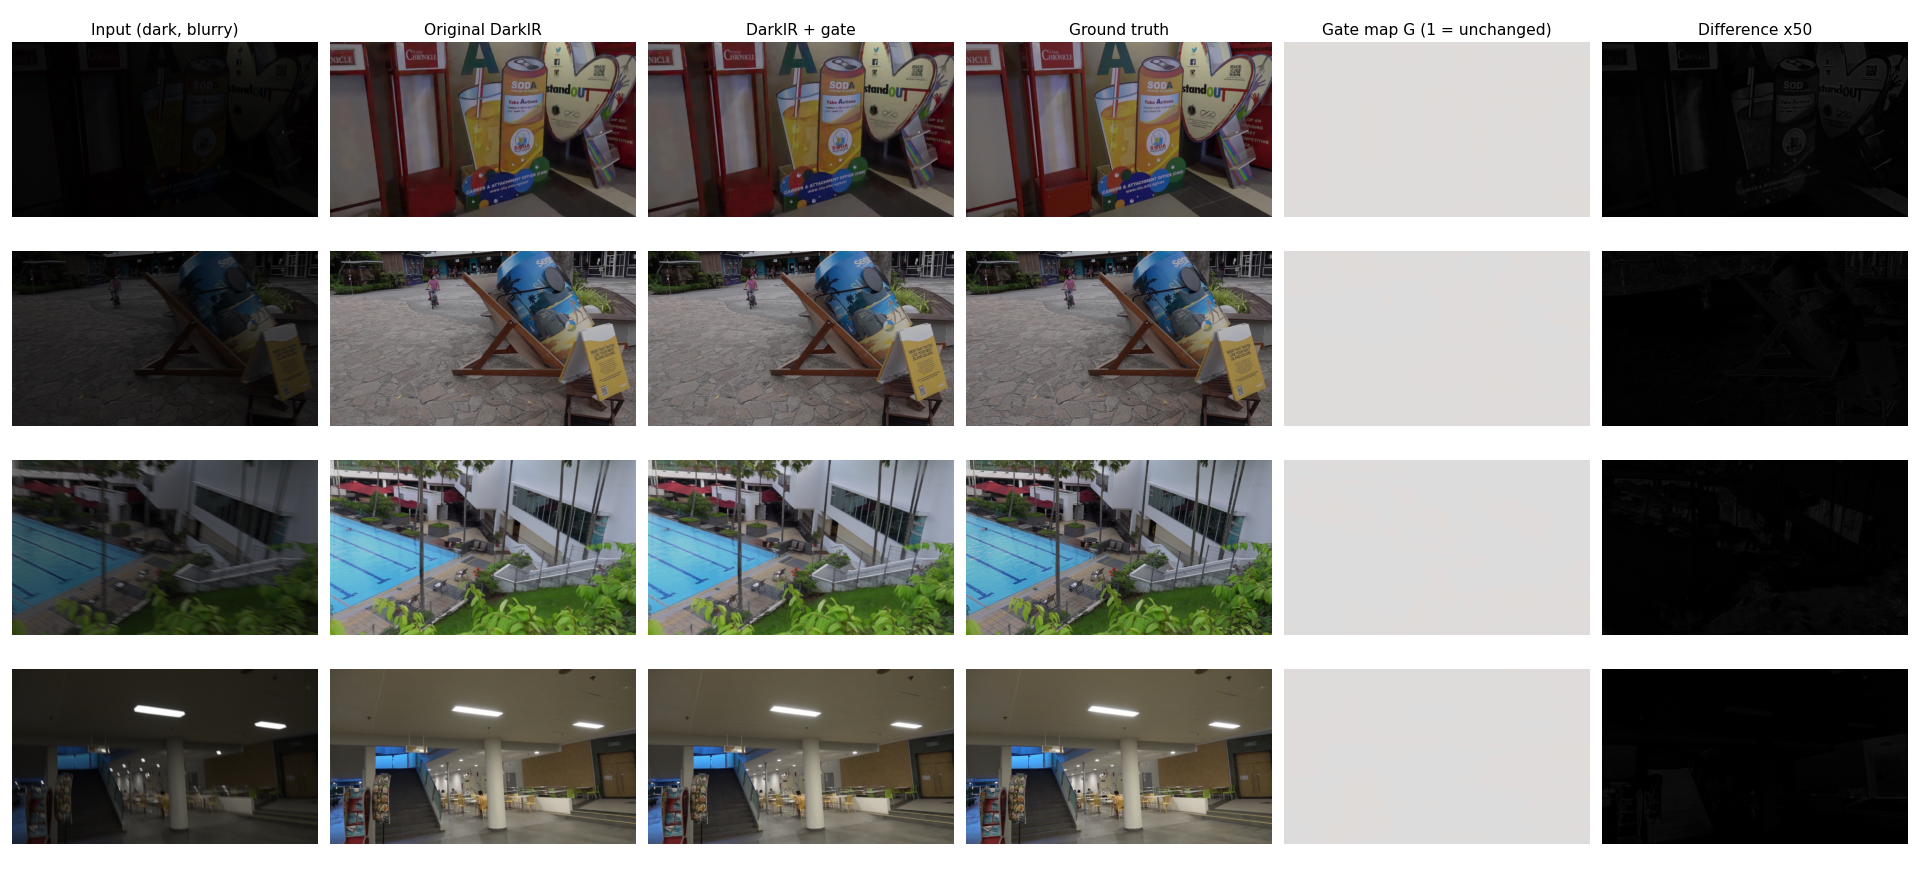
\includegraphics[width=\textwidth]{fig_gate_maps.png}
\caption{Four evenly spaced test photos, L1 gate, seed 0. Columns: input, original DarkIR, DarkIR with gate, ground truth, gate map $G$ on a 0 to 2 scale, and the absolute difference between the two outputs multiplied by 50.}
\label{fig:maps}
\end{figure*}

When the colour scale is zoomed to 0.995--1.02 (Fig.~\ref{fig:zoom}) the map is clearly not random noise, and object outlines are visible in it. Looking at these four photos we first thought that $G$ was lower in smooth areas and higher in detailed areas. To check this we measured it on 20 test photos spread through the test set, using the Pearson correlation between $G$ and two quantities: the brightness of the input photo, and the edge strength (pixel-to-pixel change) of the original model's output.

The average correlation with edge strength was $+0.03$, with single photos between $-0.30$ and $+0.23$. That is essentially no relation. The correlation with input brightness averaged $-0.27$ but changed sign from photo to photo (between $-0.96$ and $+0.77$), so there is no consistent brightness rule either. $G$ was above 1 on average in all 20 photos (photo means between 1.003 and 1.013), with single values between about 0.988 and 1.020.

So we do not claim that the gate follows detail or brightness. What we can say is that on average it applies slightly more of the last decoder block's correction, with small variations whose cause we have not found. Pearson correlation only picks up straight-line relations, so a more complicated relation may exist.

\begin{figure*}[t]
\centering
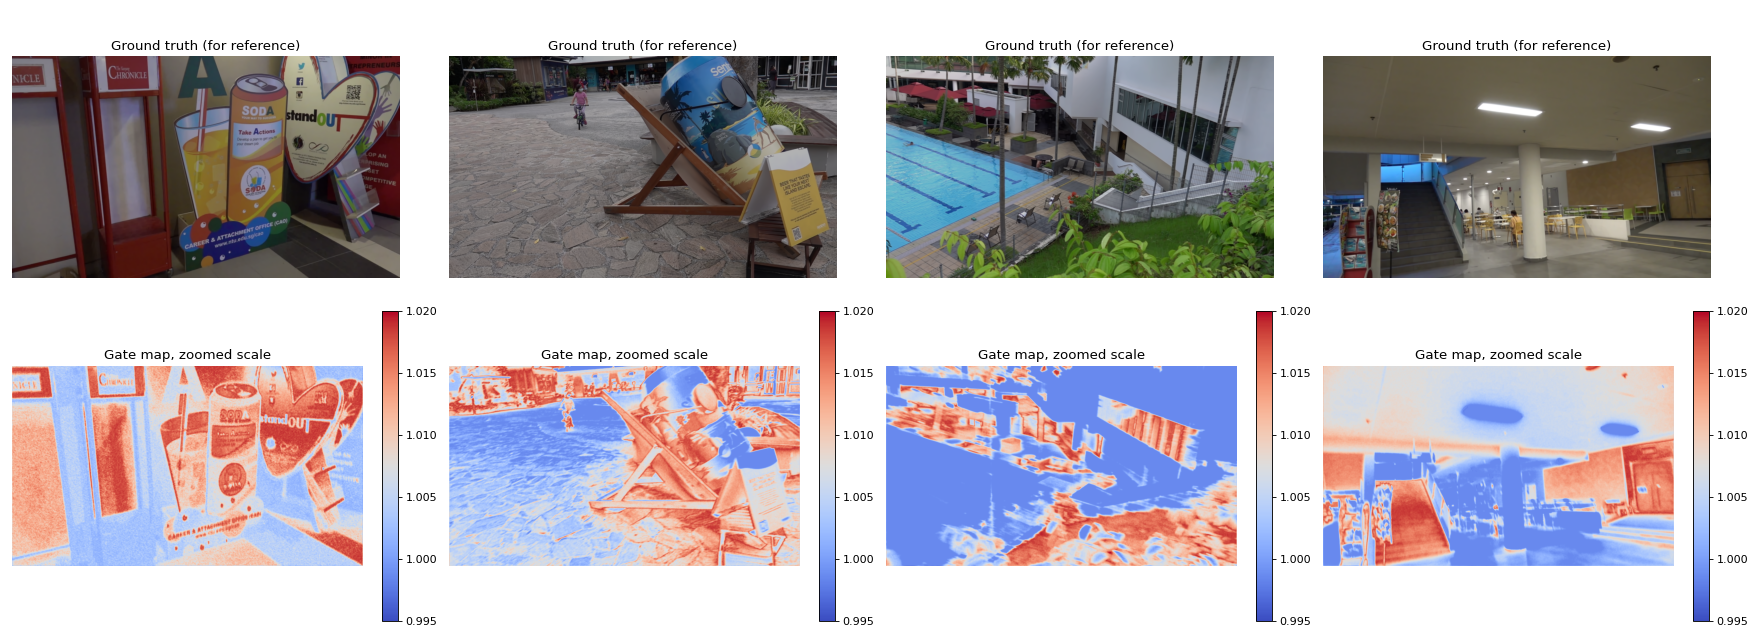
\includegraphics[width=\textwidth]{fig_gate_zoom.png}
\caption{Ground truth (top) and the gate maps of the same four photos with the colour scale zoomed to 0.995--1.02 (bottom). The whole range is only about 2\%, so the zoom exaggerates the pattern.}
\label{fig:zoom}
\end{figure*}

Since we cannot tie the pattern to a simple image property, we also cannot explain why LPIPS improved. The average $G$ is about 1.006, so a plain constant scale factor of that size might give a similar gain. We did not run this control (a gate with one learnable number instead of a map). Therefore we have not shown that the spatial variation, as opposed to a small global change, is responsible for the improvement.

\section{Experiments That Did Not Work}
We report these because they shaped the final design and because the final gain is so small.

\subsection{Fine-tuning the whole network}
Our first round fine-tuned the entire network for 10 epochs with L1 loss. There was a control without a gate and two gated versions (one gate at the last decoder stage, one at all three). On a 300-image test subset none of them improved SSIM or LPIPS over the original, and the control suffered the same loss (Table~\ref{tab:first}).

\begin{table}[t]
\caption{First round, whole network fine-tuned (300-image test subset).}
\label{tab:first}
\centering
\footnotesize
\setlength{\tabcolsep}{3pt}
\begin{tabular}{lcccr}
\toprule
Model & PSNR $\uparrow$ & SSIM $\uparrow$ & LPIPS $\downarrow$ & Params \\
\midrule
DarkIR-m (original) & 27.098 & 0.8852 & 0.1591 & 3,321,638 \\
Control, no gate & 27.144 & 0.8833 & 0.1623 & 3,321,638 \\
Gate, last stage & 27.037 & 0.8829 & 0.1628 & 3,322,231 \\
Gates, all 3 stages & 26.988 & 0.8829 & 0.1624 & 3,323,417 \\
\bottomrule
\end{tabular}
\end{table}

The PSNR difference of the control was within noise, but its SSIM and LPIPS were worse than the original. Our best explanation, which we have not proven, is that short fine-tuning with plain L1 loss on 1{,}500 pairs moves the network a little away from the authors' own training recipe. This is why the final experiments keep the network frozen.

\subsection{Training the gate longer}
We checked whether the small gains were limited by training time. The combined-loss gate was retrained for 30 epochs instead of 10 with everything else unchanged. The training loss stayed flat for all 30 epochs (0.0699 in epoch 1 and 0.0700 in epoch 30). On the 300-image subset the 30-epoch model scored PSNR 27.0849, SSIM 0.88538 and LPIPS 0.15884, against 27.0834, 0.88532 and 0.15885 for the 10-epoch model. These differences are far inside the noise, so training three times longer changed nothing. This was only checked on the subset with one seed.

\subsection{Other problems}
Training in half precision (fp16) gave invalid values (NaN) and no learning; full precision fixed this. The frozen-network gate with a 0--1 sigmoid did not learn at all (Section~III-B).

\section{Limitations}
\begin{itemize}
\item The improvements are very small (LPIPS about 0.06\% to 0.14\%) and cannot be seen by eye. They are distinguishable from noise on this test set by our informal check, but the practical benefit is negligible.
\item Only LPIPS improved clearly. We do not claim any improvement in PSNR or SSIM.
\item The combined loss contains LPIPS directly, so part of its larger LPIPS gain is expected and may not carry over to other perceptual metrics. The combined-loss gate was trained with one seed only.
\item We tried several variants and chose the next one after seeing test results of the earlier ones (for example, we tried the combined loss after seeing the L1 results). The final test numbers are therefore not completely free of selection.
\item We used one dataset (LOLBlur) with 30 test scenes, short training on a subset, and a gate at a single decoder stage. Other datasets, gate positions and more seeds were not tested.
\item The gate maps were looked at visually on 4 photos and by correlation on 20 photos, and no simple pattern was found. Without the constant-scale control we cannot say that the spatial variation matters.
\end{itemize}

\section{Conclusion}
A 593-parameter gate added to a frozen DarkIR-m gave a small and consistent LPIPS improvement on the LOLBlur test set. It was repeated over two random seeds with the L1 loss and was larger with a loss containing SSIM and LPIPS terms. On average the gate applies slightly more of the last decoder block's correction, but the effect is only about 2\%, we could not connect its pattern to detail or brightness, and it did not clearly improve PSNR or SSIM. Because the constant-scale control is missing, the result does not show that spatially adaptive restoration strength is what helps. It only shows that this small add-on gives a marginal LPIPS gain. The obvious next steps are that control, more seeds for the combined loss, and a test on other low-light datasets.

\section*{Code Availability}
The code (gate module, training and evaluation scripts, a Colab notebook and a README) is at \url{https://github.com/YOUR-USERNAME/darkir-spatial-gate}. The gate module is a subclass of the original DarkIR class and no file of the original repository is changed.

\begin{thebibliography}{00}
\bibitem{darkir} D. Feijoo, J. C. Benito, A. Garcia, and M. V. Conde, ``DarkIR: Robust low-light image restoration,'' in \textit{Proc. IEEE/CVF Conf. Computer Vision and Pattern Recognition (CVPR)}, 2025, pp. 10879--10889.
\bibitem{lednet} S. Zhou, C. Li, and C. C. Loy, ``LEDNet: Joint low-light enhancement and deblurring in the dark,'' in \textit{Proc. European Conf. Computer Vision (ECCV)}, 2022.
\bibitem{nafnet} L. Chen, X. Chu, X. Zhang, and J. Sun, ``Simple baselines for image restoration,'' in \textit{Proc. European Conf. Computer Vision (ECCV)}, 2022, pp. 17--33.
\bibitem{senet} J. Hu, L. Shen, and G. Sun, ``Squeeze-and-excitation networks,'' in \textit{Proc. IEEE Conf. Computer Vision and Pattern Recognition (CVPR)}, 2018, pp. 7132--7141.
\bibitem{lpips} R. Zhang, P. Isola, A. A. Efros, E. Shechtman, and O. Wang, ``The unreasonable effectiveness of deep features as a perceptual metric,'' in \textit{Proc. IEEE Conf. Computer Vision and Pattern Recognition (CVPR)}, 2018, pp. 586--595.
\bibitem{ssim} Z. Wang, A. C. Bovik, H. R. Sheikh, and E. P. Simoncelli, ``Image quality assessment: From error visibility to structural similarity,'' \textit{IEEE Trans. Image Process.}, vol. 13, no. 4, pp. 600--612, 2004.
\bibitem{adamw} I. Loshchilov and F. Hutter, ``Decoupled weight decay regularization,'' in \textit{Proc. Int. Conf. Learning Representations (ICLR)}, 2019.
\end{thebibliography}

\end{document}
